\documentclass[12pt]{article}

% Separate working manuscript. Canonical main.* files are unchanged.
% !TEX TS-program = xelatex
% File: preamble.tex
% Purpose: Brett Reynolds house style LaTeX preamble
% Version: 2.0.0 (December 2025 typography redesign)
%
% Usage: % !TEX TS-program = xelatex
% File: preamble.tex
% Purpose: Brett Reynolds house style LaTeX preamble
% Version: 2.0.0 (December 2025 typography redesign)
%
% Usage: % !TEX TS-program = xelatex
% File: preamble.tex
% Purpose: Brett Reynolds house style LaTeX preamble
% Version: 2.0.0 (December 2025 typography redesign)
%
% Usage: \input{.house-style/preamble.tex} in main document
%
% Compiler: XeLaTeX (default) or LuaLaTeX
%           NOT pdfLaTeX - requires fontspec for fonts

% ===========================
% FONTS
% ===========================
\usepackage{fontspec}

\setmainfont{EBGaramond}[
  Extension=.otf,
  UprightFont=*-Regular,
  ItalicFont=*-Italic,
  BoldFont=*-Bold,
  BoldItalicFont=*-BoldItalic,
  Numbers=OldStyle,
  Ligatures=TeX,
]

% IPA fallback font
\newfontfamily\ipafont{CharisSIL}[
  Extension=.ttf,
  UprightFont=*-Regular,
  ItalicFont=*-Italic,
  BoldFont=*-Bold,
  BoldItalicFont=*-BoldItalic,
]
\newcommand{\ipa}[1]{{\ipafont #1}}

% Lining figures when needed (tables, years in isolation)
\providecommand{\liningnums}[1]{{\addfontfeatures{Numbers=Lining}#1}}

% Monospace
\setmonofont{Inconsolatazi4}[
  Extension=.otf,
  UprightFont=*-Regular,
  BoldFont=*-Bold,
  Scale=MatchLowercase,
]

% ===========================
% PAGE LAYOUT
% ===========================
\usepackage[
  letterpaper,
  inner=1.25in,
  outer=1in,
  top=1in,
  bottom=1.25in,
  marginparwidth=0.6in,
]{geometry}

\usepackage[british]{babel}
\usepackage[final]{microtype}

% ===========================
% HEADINGS
% ===========================
\usepackage{titlesec}

% Section: small caps, number in margin
\titleformat{\section}
  {\normalfont\scshape}
  {\llap{\thesection\quad}}
  {0pt}
  {}

% Subsection: small caps sentence case
\titleformat{\subsection}
  {\normalfont\scshape}
  {\thesubsection\quad}
  {0pt}
  {}

% Subsubsection: upright
\titleformat{\subsubsection}
  {\normalfont}
  {\thesubsubsection\quad}
  {0pt}
  {}

% Spacing
\titlespacing*{\section}{0pt}{2ex plus 1ex minus .2ex}{1ex plus .2ex}
\titlespacing*{\subsection}{0pt}{1.5ex plus 1ex minus .2ex}{0.5ex plus .2ex}
\titlespacing*{\subsubsection}{0pt}{1ex plus 0.5ex minus .1ex}{0.3ex plus .1ex}

% ===========================
% RUNNING HEADS
% ===========================
\usepackage{fancyhdr}
\pagestyle{fancy}
\fancyhf{}
\setlength{\headheight}{13.6pt}
\renewcommand{\headrulewidth}{0pt}

% For oneside documents (most papers):
\fancyhead[L]{\small\scshape\leftmark}
\fancyhead[R]{\small\thepage}
\fancyfoot{}

% ===========================
% COLORS & HYPERLINKS
% ===========================
\usepackage{xcolor}
\definecolor{linkmaroon}{RGB}{128, 0, 32}

\usepackage{hyperref}
\hypersetup{
  colorlinks=true,
  linkcolor=linkmaroon,
  citecolor=linkmaroon,
  urlcolor=linkmaroon,
  pdfauthor={Brett Reynolds},
}

\usepackage{orcidlink}

% ===========================
% QUOTATIONS
% ===========================
\usepackage[style=american]{csquotes} % Double quotes outer (Oxford spelling kept via babel)
\MakeOuterQuote{"}

% ===========================
% SEMANTIC MACROS
% ===========================
% Terms (linguistic concepts being introduced/defined)
\newcommand{\term}[1]{\textsc{#1}}

% Mentions (words/expressions under discussion)
\newcommand{\mention}[1]{\textit{#1}}

% Mentions in headings (angle brackets instead of italics)
% Robust: headings are moving arguments (written to .toc/.aux)
\DeclareRobustCommand{\mentionhead}[1]{⟨\textup{#1}⟩}

% Object language (cited forms, foreign words)
\newcommand{\olang}[1]{\textit{#1}}

% Small-caps abbreviations for glosses
\newcommand{\abbr}[1]{\textsc{#1}}

% Cross-linguistic subscript marker
\usepackage{marvosym}
\newcommand{\crossmark}{\textsubscript{\Cross}}

% ===========================
% MATHS AND SYMBOLS
% ===========================
\usepackage{amsmath,amssymb}

% ===========================
% LINGUISTIC EXAMPLES
% ===========================
\usepackage{langsci-gb4e}
\makeatletter
\@ifundefined{noautomath}{}{\noautomath}
\makeatother

% Judgement markers
\newcommand{\ungram}[1]{*\!#1}
\newcommand{\marg}[1]{?\!#1}
\newcommand{\odd}[1]{\#\!#1}

% ===========================
% LISTS
% ===========================
\usepackage{enumitem}
\setlist{nosep, leftmargin=*}
\setlist[enumerate]{label=\arabic*.}
\setlist[itemize]{label=--}

% ===========================
% TABLES & FIGURES
% ===========================
\usepackage{booktabs}
\usepackage{array}
\usepackage{graphicx}
\graphicspath{{figures/}}

% ===========================
% BIBLIOGRAPHY
% ===========================
\usepackage[backend=biber,style=apa,natbib=true,doi=true,isbn=false,url=true]{biblatex}
\addbibresource{references.bib}
\IfFileExists{references-local.bib}{\addbibresource{references-local.bib}}{}

% Possessive citation: Author's (Year)
\newcommand{\posscite}[1]{\citeauthor{#1}'s (\citeyear{#1})}

% ===========================
% UTILITIES
% ===========================
\usepackage{xspace}
\newcommand{\eg}{e.g.,\xspace}
\newcommand{\ie}{i.e.,\xspace}
\newcommand{\etc}{etc.\xspace}
 in main document
%
% Compiler: XeLaTeX (default) or LuaLaTeX
%           NOT pdfLaTeX - requires fontspec for fonts

% ===========================
% FONTS
% ===========================
\usepackage{fontspec}

\setmainfont{EBGaramond}[
  Extension=.otf,
  UprightFont=*-Regular,
  ItalicFont=*-Italic,
  BoldFont=*-Bold,
  BoldItalicFont=*-BoldItalic,
  Numbers=OldStyle,
  Ligatures=TeX,
]

% IPA fallback font
\newfontfamily\ipafont{CharisSIL}[
  Extension=.ttf,
  UprightFont=*-Regular,
  ItalicFont=*-Italic,
  BoldFont=*-Bold,
  BoldItalicFont=*-BoldItalic,
]
\newcommand{\ipa}[1]{{\ipafont #1}}

% Lining figures when needed (tables, years in isolation)
\providecommand{\liningnums}[1]{{\addfontfeatures{Numbers=Lining}#1}}

% Monospace
\setmonofont{Inconsolatazi4}[
  Extension=.otf,
  UprightFont=*-Regular,
  BoldFont=*-Bold,
  Scale=MatchLowercase,
]

% ===========================
% PAGE LAYOUT
% ===========================
\usepackage[
  letterpaper,
  inner=1.25in,
  outer=1in,
  top=1in,
  bottom=1.25in,
  marginparwidth=0.6in,
]{geometry}

\usepackage[british]{babel}
\usepackage[final]{microtype}

% ===========================
% HEADINGS
% ===========================
\usepackage{titlesec}

% Section: small caps, number in margin
\titleformat{\section}
  {\normalfont\scshape}
  {\llap{\thesection\quad}}
  {0pt}
  {}

% Subsection: small caps sentence case
\titleformat{\subsection}
  {\normalfont\scshape}
  {\thesubsection\quad}
  {0pt}
  {}

% Subsubsection: upright
\titleformat{\subsubsection}
  {\normalfont}
  {\thesubsubsection\quad}
  {0pt}
  {}

% Spacing
\titlespacing*{\section}{0pt}{2ex plus 1ex minus .2ex}{1ex plus .2ex}
\titlespacing*{\subsection}{0pt}{1.5ex plus 1ex minus .2ex}{0.5ex plus .2ex}
\titlespacing*{\subsubsection}{0pt}{1ex plus 0.5ex minus .1ex}{0.3ex plus .1ex}

% ===========================
% RUNNING HEADS
% ===========================
\usepackage{fancyhdr}
\pagestyle{fancy}
\fancyhf{}
\setlength{\headheight}{13.6pt}
\renewcommand{\headrulewidth}{0pt}

% For oneside documents (most papers):
\fancyhead[L]{\small\scshape\leftmark}
\fancyhead[R]{\small\thepage}
\fancyfoot{}

% ===========================
% COLORS & HYPERLINKS
% ===========================
\usepackage{xcolor}
\definecolor{linkmaroon}{RGB}{128, 0, 32}

\usepackage{hyperref}
\hypersetup{
  colorlinks=true,
  linkcolor=linkmaroon,
  citecolor=linkmaroon,
  urlcolor=linkmaroon,
  pdfauthor={Brett Reynolds},
}

\usepackage{orcidlink}

% ===========================
% QUOTATIONS
% ===========================
\usepackage[style=american]{csquotes} % Double quotes outer (Oxford spelling kept via babel)
\MakeOuterQuote{"}

% ===========================
% SEMANTIC MACROS
% ===========================
% Terms (linguistic concepts being introduced/defined)
\newcommand{\term}[1]{\textsc{#1}}

% Mentions (words/expressions under discussion)
\newcommand{\mention}[1]{\textit{#1}}

% Mentions in headings (angle brackets instead of italics)
% Robust: headings are moving arguments (written to .toc/.aux)
\DeclareRobustCommand{\mentionhead}[1]{⟨\textup{#1}⟩}

% Object language (cited forms, foreign words)
\newcommand{\olang}[1]{\textit{#1}}

% Small-caps abbreviations for glosses
\newcommand{\abbr}[1]{\textsc{#1}}

% Cross-linguistic subscript marker
\usepackage{marvosym}
\newcommand{\crossmark}{\textsubscript{\Cross}}

% ===========================
% MATHS AND SYMBOLS
% ===========================
\usepackage{amsmath,amssymb}

% ===========================
% LINGUISTIC EXAMPLES
% ===========================
\usepackage{langsci-gb4e}
\makeatletter
\@ifundefined{noautomath}{}{\noautomath}
\makeatother

% Judgement markers
\newcommand{\ungram}[1]{*\!#1}
\newcommand{\marg}[1]{?\!#1}
\newcommand{\odd}[1]{\#\!#1}

% ===========================
% LISTS
% ===========================
\usepackage{enumitem}
\setlist{nosep, leftmargin=*}
\setlist[enumerate]{label=\arabic*.}
\setlist[itemize]{label=--}

% ===========================
% TABLES & FIGURES
% ===========================
\usepackage{booktabs}
\usepackage{array}
\usepackage{graphicx}
\graphicspath{{figures/}}

% ===========================
% BIBLIOGRAPHY
% ===========================
\usepackage[backend=biber,style=apa,natbib=true,doi=true,isbn=false,url=true]{biblatex}
\addbibresource{references.bib}
\IfFileExists{references-local.bib}{\addbibresource{references-local.bib}}{}

% Possessive citation: Author's (Year)
\newcommand{\posscite}[1]{\citeauthor{#1}'s (\citeyear{#1})}

% ===========================
% UTILITIES
% ===========================
\usepackage{xspace}
\newcommand{\eg}{e.g.,\xspace}
\newcommand{\ie}{i.e.,\xspace}
\newcommand{\etc}{etc.\xspace}
 in main document
%
% Compiler: XeLaTeX (default) or LuaLaTeX
%           NOT pdfLaTeX - requires fontspec for fonts

% ===========================
% FONTS
% ===========================
\usepackage{fontspec}

\setmainfont{EBGaramond}[
  Extension=.otf,
  UprightFont=*-Regular,
  ItalicFont=*-Italic,
  BoldFont=*-Bold,
  BoldItalicFont=*-BoldItalic,
  Numbers=OldStyle,
  Ligatures=TeX,
]

% IPA fallback font
\newfontfamily\ipafont{CharisSIL}[
  Extension=.ttf,
  UprightFont=*-Regular,
  ItalicFont=*-Italic,
  BoldFont=*-Bold,
  BoldItalicFont=*-BoldItalic,
]
\newcommand{\ipa}[1]{{\ipafont #1}}

% Lining figures when needed (tables, years in isolation)
\providecommand{\liningnums}[1]{{\addfontfeatures{Numbers=Lining}#1}}

% Monospace
\setmonofont{Inconsolatazi4}[
  Extension=.otf,
  UprightFont=*-Regular,
  BoldFont=*-Bold,
  Scale=MatchLowercase,
]

% ===========================
% PAGE LAYOUT
% ===========================
\usepackage[
  letterpaper,
  inner=1.25in,
  outer=1in,
  top=1in,
  bottom=1.25in,
  marginparwidth=0.6in,
]{geometry}

\usepackage[british]{babel}
\usepackage[final]{microtype}

% ===========================
% HEADINGS
% ===========================
\usepackage{titlesec}

% Section: small caps, number in margin
\titleformat{\section}
  {\normalfont\scshape}
  {\llap{\thesection\quad}}
  {0pt}
  {}

% Subsection: small caps sentence case
\titleformat{\subsection}
  {\normalfont\scshape}
  {\thesubsection\quad}
  {0pt}
  {}

% Subsubsection: upright
\titleformat{\subsubsection}
  {\normalfont}
  {\thesubsubsection\quad}
  {0pt}
  {}

% Spacing
\titlespacing*{\section}{0pt}{2ex plus 1ex minus .2ex}{1ex plus .2ex}
\titlespacing*{\subsection}{0pt}{1.5ex plus 1ex minus .2ex}{0.5ex plus .2ex}
\titlespacing*{\subsubsection}{0pt}{1ex plus 0.5ex minus .1ex}{0.3ex plus .1ex}

% ===========================
% RUNNING HEADS
% ===========================
\usepackage{fancyhdr}
\pagestyle{fancy}
\fancyhf{}
\setlength{\headheight}{13.6pt}
\renewcommand{\headrulewidth}{0pt}

% For oneside documents (most papers):
\fancyhead[L]{\small\scshape\leftmark}
\fancyhead[R]{\small\thepage}
\fancyfoot{}

% ===========================
% COLORS & HYPERLINKS
% ===========================
\usepackage{xcolor}
\definecolor{linkmaroon}{RGB}{128, 0, 32}

\usepackage{hyperref}
\hypersetup{
  colorlinks=true,
  linkcolor=linkmaroon,
  citecolor=linkmaroon,
  urlcolor=linkmaroon,
  pdfauthor={Brett Reynolds},
}

\usepackage{orcidlink}

% ===========================
% QUOTATIONS
% ===========================
\usepackage[style=american]{csquotes} % Double quotes outer (Oxford spelling kept via babel)
\MakeOuterQuote{"}

% ===========================
% SEMANTIC MACROS
% ===========================
% Terms (linguistic concepts being introduced/defined)
\newcommand{\term}[1]{\textsc{#1}}

% Mentions (words/expressions under discussion)
\newcommand{\mention}[1]{\textit{#1}}

% Mentions in headings (angle brackets instead of italics)
% Robust: headings are moving arguments (written to .toc/.aux)
\DeclareRobustCommand{\mentionhead}[1]{⟨\textup{#1}⟩}

% Object language (cited forms, foreign words)
\newcommand{\olang}[1]{\textit{#1}}

% Small-caps abbreviations for glosses
\newcommand{\abbr}[1]{\textsc{#1}}

% Cross-linguistic subscript marker
\usepackage{marvosym}
\newcommand{\crossmark}{\textsubscript{\Cross}}

% ===========================
% MATHS AND SYMBOLS
% ===========================
\usepackage{amsmath,amssymb}

% ===========================
% LINGUISTIC EXAMPLES
% ===========================
\usepackage{langsci-gb4e}
\makeatletter
\@ifundefined{noautomath}{}{\noautomath}
\makeatother

% Judgement markers
\newcommand{\ungram}[1]{*\!#1}
\newcommand{\marg}[1]{?\!#1}
\newcommand{\odd}[1]{\#\!#1}

% ===========================
% LISTS
% ===========================
\usepackage{enumitem}
\setlist{nosep, leftmargin=*}
\setlist[enumerate]{label=\arabic*.}
\setlist[itemize]{label=--}

% ===========================
% TABLES & FIGURES
% ===========================
\usepackage{booktabs}
\usepackage{array}
\usepackage{graphicx}
\graphicspath{{figures/}}

% ===========================
% BIBLIOGRAPHY
% ===========================
\usepackage[backend=biber,style=apa,natbib=true,doi=true,isbn=false,url=true]{biblatex}
\addbibresource{references.bib}
\IfFileExists{references-local.bib}{\addbibresource{references-local.bib}}{}

% Possessive citation: Author's (Year)
\newcommand{\posscite}[1]{\citeauthor{#1}'s (\citeyear{#1})}

% ===========================
% UTILITIES
% ===========================
\usepackage{xspace}
\newcommand{\eg}{e.g.,\xspace}
\newcommand{\ie}{i.e.,\xspace}
\newcommand{\etc}{etc.\xspace}

\usepackage{xurl}
\usepackage[normalem]{ulem}
\setlength{\ULdepth}{1.8pt}
\setlength{\emergencystretch}{3em}
\setlength{\headheight}{14pt}
\newcommand{\exmention}[1]{\mention{#1}}
\newcommand{\exfocus}[1]{\uline{#1}}
\newcommand{\intj}[1]{\textsc{interjection\textsubscript{#1}}}
\newcommand{\intjshort}[1]{Intj\textsubscript{#1}}
\addbibresource{inquiry-relative-categories.bib}

% Publisher-verified correction without changing the shared bibliography.
\DeclareSourcemap{
  \maps[datatype=bibtex]{
    \map[overwrite=true]{
      \step[fieldsource=entrykey, match=\regexp{\Aunuabonahdaniel2020\Z}, final]
      \step[fieldset=doi, fieldvalue={10.1016/j.pragma.2020.04.004}]
    }
  }
}

\newif\ifblind
\blindfalse
\ifblind
\DeclareSourcemap{
  \maps[datatype=bibtex]{
    \map[overwrite=true]{
      \step[fieldsource=entrykey, match=\regexp{\Areynolds}, final]
      \step[fieldset=author, fieldvalue={Author}]
      \step[fieldset=title, fieldvalue={[Title removed for anonymous review]}]
      \step[fieldset=note, null]
      \step[fieldset=url, null]
      \step[fieldset=doi, null]
    }
  }
}
\fi
\hypersetup{
  pdftitle={Inquiry-Relative Categories: Evidence Supplement},
  pdfkeywords={inquiry-relative categories, category pluralism, projectibility, interjections, sign-types, path dependence},
}
\ifblind
\hypersetup{pdfauthor={}}
\else
\hypersetup{pdfauthor={Brett Reynolds}}
\fi
\title{Inquiry-Relative Categories:\\Evidence Supplement}
\ifblind
\author{[Author removed for blind review]}
\else
\author{Brett Reynolds \orcidlink{0000-0003-0073-7195}%
\thanks{Contact: \href{mailto:brett.reynolds@humber.ca}{brett.reynolds@humber.ca}}\\
Humber Polytechnic \& University of Toronto}
\fi
\date{\today}

\begin{document}
\maketitle


This supplement preserves the measurement records accompanying
\href{inquiry-relative-categories.pdf}{Inquiry-Relative Categories: English
Interjections as a Worked Case}. It distinguishes retained descriptions
from invalid confirmatory interpretations. No new corpus coding or model
fit is reported. The older diagnostic labels in Section~C are retained
to identify archived outputs; they don't allocate one category to each
field in the main paper.

\begingroup\raggedright
Sections~A--C document the GloWbE, derivative, and \mention{fie} analyses.
Section~D preserves the COHA inventory comparison. Numerical outputs from
invalid analyses remain solely as records of what the pipelines produced.
All audits refer to repository revision
\texttt{074dfb44cef5b18d292ac176ba5acbfedc76e3b1}.

\par\endgroup

\appendix

\section[GloWbE measurement and models]{GloWbE measurement and model comparisons}
\label{app:conditioning}

\subsection{Data and measurement}

Frequency counts for 18 items were extracted from GloWbE \citep{daviesfuchs2015}: 1.9 billion words across 20 countries. The items are the 10 most frequent interjection-tagged forms (\mention{yes}, \mention{no}, \mention{oh}, \mention{yeah}, \mention{hi}, \mention{hey}, \mention{wow}, \mention{hello}, \mention{ah}, \mention{ha}), three regional forms (\mention{lah}, \mention{yaar}, \mention{haba}), semi-regional \mention{eh}, boundary items \mention{cheers} and \mention{bye}, and fillers \mention{um} and \mention{uh}. Core counts are tag-restricted; regional counts are raw strings because the tagger doesn't recognize the relevant uses. Neither measure independently identifies the grammatical, expressive, depictive, or interactional groupings discussed in the main paper.

Country is assigned to a page rather than a speaker. Assignment uses Google's region function: country domains provide a direct cue, but for \texttt{.com} and \texttt{.org} sites Google \enquote{relies on several heuristics, including 1) the IP address for the web server, 2) who links to that website, and 3) who visits the website} \citep[4]{daviesfuchs2015}. 

Davies and Fuchs themselves question \enquote{how well Google has correctly identified web sites by country}. The page list was seeded through Google searches for \enquote{hundreds of very high frequency 3-grams (three word strings)} from the Corpus of Contemporary American English (p.~4), anchoring the sampling frame to American frequency data. Country differences may reflect genre mix, internet ecology, and sampling alongside linguistic variation.

Automatic tagging adds another measurement layer. An overall error rate doesn't warrant comparisons if validity varies by country \citep{reynolds2026didcorpus}. Concordance coding estimates precision, the proportion of tagged hits that are genuine, not recall, the proportion of genuine tokens retrieved. Neither \mention{haba} nor \mention{yaar} receives an interjection tag. All 373 Nigerian \mention{haba} hits are tagged as common or proper nouns, with 65\% on a reading including the proper noun. The raw-string regional counts can overstate frequency while a tag-restricted query misses these forms entirely.

\subsection{Geographic distributions}

Regional concentration is clear in the raw strings: \mention{lah} occurs at 9.35 per million words in Malaysia and 6.72 in Singapore, and \mention{yaar} at 2.88 in Pakistan and 2.33 in India, with near-zero rates elsewhere. Nigeria's 373 \mention{haba} hits give an upper bound of about 9 per million. Inspecting hits, counting five spellings, and excluding Nigerian Pidgin, indigenous-language material, and duplicates, \textcite[69]{unuabonahdaniel2020} report 248 tokens, or 5.8 per million. The gap illustrates why raw strings and tagged counts aren't directly comparable.

Among the core items, \mention{ah} has the largest cross-country coefficient of variation (CV; standard deviation divided by mean), 0.71: Singapore's 60.42 and Jamaica's 53.16 per million are about eight times Kenya's 7.62. For \mention{yeah}, CV is 0.55 and the United States--Tanzania comparison is approximately 6:1 (103.78 versus 16.85). \mention{Yes} and \mention{no} have lower CVs, 0.21--0.22. The fillers \mention{um} and \mention{uh} have CVs of 0.61 and 0.76, and \mention{bye} has 0.61.

Bootstrap intervals resample the twenty observed country sections. They describe sensitivity to that resampling, not sampling uncertainty over all English-speaking communities: the sections aren't a random sample of such communities. The \mention{yes}/\mention{no} intervals lie below those of eleven of the thirteen other nonregional items, overlapping only \mention{hello} and \mention{ha}. This supports their comparatively low observed dispersion. 

The remaining marginal intervals overlap; that doesn't establish equal dispersion or settle pairwise differences. A ranking would require paired contrasts within resamples. Regional concentration is better represented by the counts: when a form is absent from eighteen sections, resampling can sharply alter the mean and CV. For \mention{lah}, the interval runs from 0.89 to 4.27.

\begin{figure}[ht]
  \centering
  % Crop the archived title/subtitle: its median label is misleading because
  % stat_summary is evaluated within each item facet, with one rate per country.
  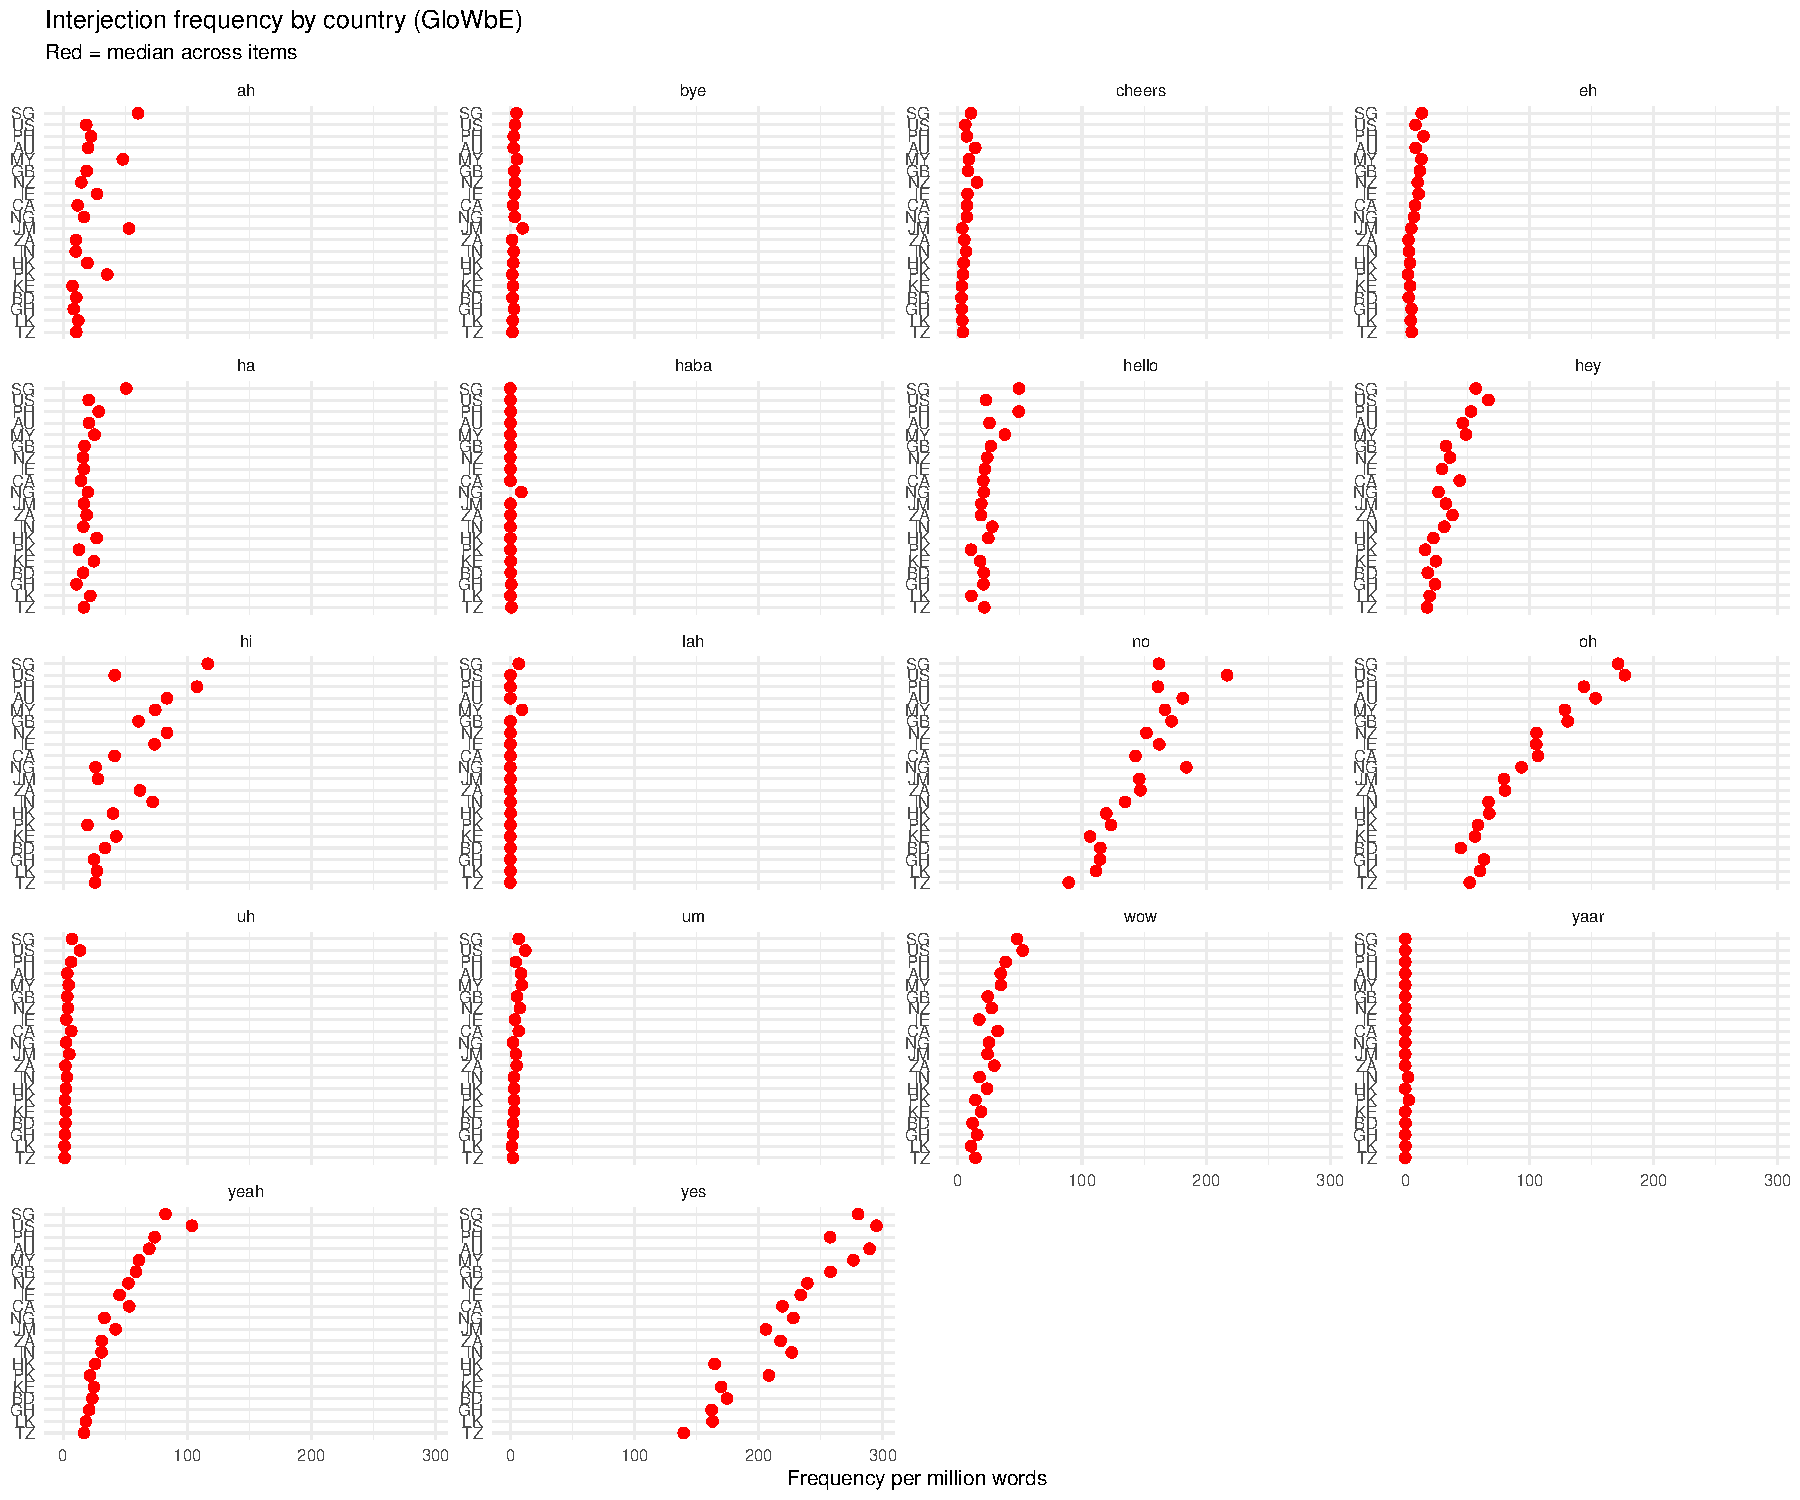
\includegraphics[width=\textwidth,trim=0 0 0 34,clip]{country-variation.pdf}
  \caption{Frequency per million words across 20 GloWbE country sections. Red points give the rate for each country--item combination. Regional strings (\mention{lah}, \mention{yaar}, \mention{haba}) concentrate in one or two countries; \mention{yes} and \mention{no} have comparatively low dispersion. Tagging and raw-string validity differ by item and country, as the audit below documents.}
  \label{fig:country-variation}
\end{figure}

\subsection{Concordance audit and sensitivity}

The tagger misses relevant regional uses, and even recognized items can contain false positives. An initial twenty-token check of tagged \mention{ha} in Kenya and Tanzania retained six and eight interjections respectively; most other hits abbreviated \term{hectare} in agricultural and development prose. Applying the Kenyan estimate reduces 24.9 tokens per million to about 7.5 and moves Kenya from fifth to nineteenth among the twenty sections. This preliminary estimate differs from the fuller audit below.

The \mention{ha} audit also requires an explicit decision about laughter. Iterated \mention{HA! HA!} may represent laughter, closer to eye dialect than a lexical item, whereas sarcastic or sceptical \mention{ha} is an interjectional use. Written data make the distinction harder, and digital \mention{haha} may itself be conventionalized. This decision doesn't exclude imitative forms in principle; imitation is one proposed recruitment route. The reported counts include iterated laughter.

The fuller twenty-section audit uses a deterministic regular-expression
screen, implemented in \path{analysis/filter-ha-concordance.py}. Its rules
inspect reduplication, laughter words, punctuation, units, numbers, names,
and typography. All twenty rows of \path{data/ha-validity-rates.csv}
reproduce those automated assignments. The precision estimates below are
conditional on that screen; they aren't independently adjudicated
country-wide proportions of genuine interjections.

The screen was checked and tuned against forty previously labelled
Kenyan and Tanzanian examples. The adding commit records changes to
the rules after inspecting errors on those examples. Its 39/40 agreement
concerns the binary interjection decision; exact agreement across the
five labels is 37/40. These are development-set comparisons. They don't
establish held-out accuracy or comparable error rates across all twenty
sections, and the archive doesn't establish the initial labeller's identity.

Under the screen, laughter accounts for 51.5\% of sampled US tagged
\mention{ha} and 63.0\% of sampled British tagged \mention{ha}. Table~\ref{tab:ha-sensitivity}
separates six treatments of laughter and unclear cases
\citep[cf.][]{gelman2014statcrisis}. Here \term{unpooled} means rates adjusted
using each section's screen-derived proportion without shrinkage; it
doesn't mean the original tagged rates. The original uncorrected
coefficient of variation is approximately 0.412.

\begin{table}[htbp]
\centering
\small
\caption{Sensitivity of adjusted \mention{ha} rates to screen-based inclusion rules.
Unclear cases receive weight 0, 0.5, or 1. CV is the standard deviation
divided by the mean of the twenty section rates.}
\label{tab:ha-sensitivity}
\begin{tabular}{@{}llrrrr@{}}
\toprule
 & Unclear & \multicolumn{2}{c}{CV} & \multicolumn{2}{c}{Kenya rank} \\
\cmidrule(lr){3-4}\cmidrule(l){5-6}
Laughter & weight & Unpooled & Pooled & Unpooled & Pooled \\
\midrule
Included & 0   & 0.396 & 0.395 & 15 & 15 \\
Included & 0.5 & 0.420 & 0.419 & 15 & 14 \\
Included & 1   & 0.446 & 0.445 & 15 & 15 \\
Excluded & 0   & 0.793 & 0.778 & 15 & 15 \\
Excluded & 0.5 & 0.810 & 0.796 & 15 & 15 \\
Excluded & 1   & 0.828 & 0.817 & 16 & 16 \\
\bottomrule
\end{tabular}
\end{table}

Kenya falls from fifth in the original tagged rates to fifteenth or
sixteenth across the six unpooled specifications; pooled ranks range
from fourteenth to sixteenth. The downward movement survives these
choices, but its exact rank doesn't. The laughter-inclusive adjusted
CVs also differ from the original uncorrected 0.412.

With laughter included and unclear cases excluded, the screen retains
34.5\% of sampled hits in Bangladesh and 84.0\% in Great Britain.
It identifies \term{hectare} as a major contaminant in East Africa and
South Asia, and names as relevant in Singapore, where it assigns 6.1\%
to \term{hectare}. These percentages describe the screen's output.
Their accuracy as linguistic measurements requires separate validation.

Pooling uses the exported sample sizes: 1,000 US rows and 200 Ghanaian
rows, compared with corpus totals of 8,016 and 420 tagged occurrences.
The twenty exports contain 16,197 rows. Shrinkage changes the proportions
by about 0.6 percentage points at most across the six specifications.
The small change reflects estimated binomial sampling variation under
the pooling model; it doesn't bound classification error or uncertainty
about the representativeness of the exported contexts.

Between-section differences in screen-derived proportions exceed the
binomial variation represented by that calculation. Whether they exceed
all measurement error is unknown. The sensitivity choices also don't
cover every possible screen error, and false-negative retrieval remains
unmeasured. The relevant code and output are
\path{analysis/pool-ha-rates.py} and
\path{analysis/hand-extracted/ha-pooled-multiverse.csv}.

Spelling variants introduce another country-dependent error. Raw \mention{ya} and \mention{yeh} look like variants of \mention{yeah}, but they concentrate where substrate words are homographs: \mention{ya} peaks in Tanzania (19.5 per million) and Malaysia (13.9), and \mention{yeh} in Singapore (5.6), Pakistan (4.9), and India (4.9). No \mention{yeh} token carries the interjection tag. Pooling both strings with \mention{yeah} reduces its CV from 0.55 to 0.46 while importing non-English tokens unevenly, so the analysis keeps them separate.

Adding \mention{umm}, \mention{ummm}, and \mention{ummmm} to \mention{um} changes its CV from 0.61 to 0.60 with Pakistan excluded, but to 0.72 with Pakistan included. Pakistan returns nearly eight times as many \mention{umm} as \mention{um} tokens, against a median ratio of about a third elsewhere. In a twenty-token Pakistani sample, nineteen are the Arabic teknonym \mention{Umm}, as in \mention{Umm Salama}, from hadith or biographical material; the twentieth mentions the filler. Raw-string lengthening thus measures substrate homography as well as orthographic variation.

Regional forms face the same problem. Hand-coding sixty-nine \mention{yaar} hits puts the English-matrix rate at roughly 60\% in Pakistan and 65\% in India; other hits include Tamil \mention{yaar} \enquote{who}, names, and Roman-script Hindi or Urdu. The relevant twenty-token samples are too coarse for correction, but establish that raw rates are upper bounds. Raw \mention{yes}, \mention{no}, \mention{ha}, \mention{ah}, \mention{oh}, \mention{well}, \mention{right}, and \mention{like} likewise include clausal, quoted, discourse-marker, literary, or noisy uses. The audit establishes a measurement result: validity varies across countries, so pooled frequencies can conceal measurement differences alongside linguistic differences.

\subsection{Model specification}

Four Bayesian negative binomial models were fitted in \texttt{brms}~2.23 in R, with four chains of 2,000 iterations, including 1,000 warmup iterations. Models m0--m2 request pointwise leave-one-out cross-validation (LOO), with \texttt{reloo} enabling exact refits for problematic observations; this is not a record of 360 exact refits. Exploratory m3 is assessed through Pareto-smoothed importance sampling (PSIS) diagnostics only.

\begin{quote}
\small \noindent\texttt{m0} (unconditional):\\ \texttt{count \textasciitilde{} 1 + offset(log(words\_m)) + (1~|~item)}

\noindent\parbox{\linewidth}{\texttt{m1} (conditioned):\\ \texttt{count \textasciitilde{} 1 + offset(log(words\_m)) +}\\ \texttt{(1~|~item) + (1~|~country)}}

\noindent\parbox{\linewidth}{\texttt{m2} (item type):\\ \texttt{count \textasciitilde{} 1 + item\_type + offset(log(words\_m)) +}\\ \texttt{(1~|~item) + (1~|~country)}}

\noindent\parbox{\linewidth}{\texttt{m3} (exploratory):\\ \texttt{count \textasciitilde{} 1 + item\_type + offset(log(words\_m)) +}\\ \texttt{(1~|~item) + (1~+~item\_type~||~country)}}
\end{quote}

The held-out observation is one country--item aggregate from the 18-item
by 20-country design. Its training data retain the same item in nineteen
other countries and seventeen other items in the same country. The target
is an omitted cell within that observed design, with its corpus-size
offset supplied. It isn't an unseen country, an unseen item, a later
period, or a newly categorized sign-type.

The country intercept in m1 estimates an overall frequency shift across items, not an item-specific country effect. Model m3 adds country-varying slopes by item type, but the sparse type cells~-- semi-regional: 1 item; boundary: 2; filler: 2; regional: 3~-- provide little support for those slopes. Neither model estimates grammatical availability separately from preference or frequency of relevant occasions.

\subsection{Results}

The archived pointwise LOO comparisons for models m0--m2 are:

\begin{center}
\begin{tabular}{lrr}
  \hline
  Model & ELPD diff & SE diff \\
  \hline
  m1 (conditioned) & 0.0 & 0.0 \\
  m2 (item type) & $-$9.3 & 7.9 \\
  m0 (unconditional) & $-$17.9 & 13.3 \\
  \hline
\end{tabular}
\end{center}

The country-conditioned model has the highest expected log predictive density (ELPD) point estimate, with an imprecise advantage over m0: $\Delta$ELPD = 17.9, standard error 13.3. Adding item type doesn't improve the point estimate for this omitted-cell task. Item intercepts already receive information from the same items elsewhere; the comparison therefore doesn't settle whether type helps predict an unfamiliar item. Model m3 isn't formally ranked because nine observations retain Pareto $k > 0.7$ after moment matching, leaving its PSIS estimates unstable.

In m1, the country standard deviation is 0.44 (95\% credible interval [CrI]: 0.28--0.65), against an item standard deviation of 2.07 (1.49--2.96), a ratio of 4.7:1. The country interval describes estimated variation under the model; its positive bounds aren't independent evidence against an absent effect, since standard deviations are constrained to be nonnegative. The predictive comparison and descriptive frequencies supply the relevant evidence. With 18 items $\times$ 20 countries = 360 observations, the ELPD uncertainty remains substantial.

To propagate the \mention{ha} precision estimates, each country's count was thinned by draws from its \textsc{beta} posterior, leaving the other seventeen items unchanged, and m0 and m1 were refitted. Within this sensitivity analysis, country standard deviation changes from 0.42 to 0.44 with iterated laughter included and 0.45 with it excluded; the model-comparison values change from 28.8 to 26.9 and 28.5. These approximate leave-one-out values support only an internal comparison, not replacement of the pointwise LOO results above. The draws represent binomial uncertainty in screen-derived proportions; they don't propagate unknown screen errors or establish sample representativeness. Precision correction leaves recall unidentified.

The evidence supports geographic concentration of particular strings and additional overall country variation in these measured frequencies. It doesn't establish social indexing, item-type-specific conditioning, category-boundary decomposition, or a process maintaining the interjectional profile. The audit explains why those stronger interpretations require independently validated uses and comparable contexts.

\clearpage

\section[Semantic residue in COHA]{Audit of the semantic-residue analysis in COHA}
\label{app:morphgain}

\subsection{Design and extraction}

The morphology-gain study was preregistered before confirmatory extraction and coding, after disclosed feasibility queries (\texttt{f1a2193}, 27 May 2026). Its fixed COHA source families were \mention{wow}, \mention{boo}, \mention{ooh}, and \mention{shoo}, over 1820--2019. The target derivatives were \mention{wowed}, \mention{wowing}, \mention{wows}; \mention{booed}, \mention{booing}, \mention{boos}; \mention{oohed}, \mention{oohing}, \mention{oohs}; and \mention{shooed}, \mention{shooing}, \mention{shoos}. Bare forms were excluded. Extraction on 27 May 2026 used key-word-in-context (KWIC) exports; chart requests for \mention{oohed} and \mention{oohing} failed, but their KWIC exports loaded. The extraction summary records minor chart/KWIC count discrepancies.

The go/no-go threshold required 20 analyzable derivatives and two decades with at least three each. The archived pipeline marked all families as passing the extraction threshold (GO):

\begin{center}
\begin{tabular}{lrrl}
  \toprule
  Family & Included tokens & Decades with 3+ & Status \\
  \midrule
  \mention{boo} & 364 & 10 & GO \\
  \mention{ooh} & 52 & 6 & GO \\
  \mention{shoo} & 410 & 13 & GO \\
  \mention{wow} & 143 & 9 & GO \\
  \bottomrule
\end{tabular}
\end{center}

\subsection{Intended measures and implementation}

The intended confirmatory measures were VP-head syntax and semantic residue: impressed or evaluative response for \mention{wow}, disapproval or contempt for \mention{boo}, appreciative or surprised response for \mention{ooh}, and directive away-sending for \mention{shoo}. Secondary codes concerned interactional residue~-- recognizable response, uptake, display, or direction~-- and a recoverable target, object, addressee, or stimulus.

An implementation audit changes the evidential status of the results. The archived primary-coding script first applies exclusion rules, then assigns both \texttt{verbal\_syntax = 1} and \texttt{semantic\_residue = 1} to every retained row. The exclusion rules were intended to select verbal uses; their accuracy can't be inferred from the syntax code automatically assigned to every retained row. The resulting file contains 1,462 rows: 969 included and 493 excluded. Semantic persistence wasn't independently measured in this primary coding pass; it was assigned by the pipeline. The outputs below don't constitute a confirmatory result.

Even independently established source content would need separating from expressive meaning type. A verb can describe or cause the response expressed by its source interjection without contributing use-conditionally itself. \mention{The performance wowed us} illustrates that distinction. Continuity of source-associated content would support a limited historical relation, not continued membership in an expressive category.

\subsection{Archived outputs and their limits}

The confirmatory window began with the earliest decade containing at least three included derivatives and extended until it contained ten. Success required both confirmatory codes; the preregistered support rule placed the lower Jeffreys 95\% interval bound above 0.5. The pipeline produced:

\begin{center}
\begin{tabular}{lrlrrl}
  \toprule
  Family & Tokens & Window & $n$ & Assigned successes & Jeffreys 95\% CI \\
  \midrule
  \mention{boo} & 364 & 1920s & 17 & 17 & [0.865, 1.000] \\
  \mention{ooh} & 52 & 1960s--1980s & 10 & 10 & [0.783, 1.000] \\
  \mention{shoo} & 410 & 1890s--1900s & 16 & 16 & [0.857, 1.000] \\
  \mention{wow} & 143 & 1930s--1940s & 11 & 11 & [0.800, 1.000] \\
  \bottomrule
\end{tabular}
\end{center}

All four outputs meet the numerical rule because the semantic outcome was fixed for retained rows. The secondary diachronic model wasn't estimated because the assigned residue variable had no variation. These primary-pipeline records preserve the preregistered attempt; they establish neither semantic persistence nor a general tendency for interjections to acquire morphology or syntax.

\subsection{Reliability record and files}

The archived 10\% reliability sample contains 97 retained rows (seed 2026). Both comparison files are constant for inclusion, VP-head status, and semantic residue, so their agreement is 1.000 but Cohen's $\kappa$ is undefined. The reliability script instead returned 1.000 when expected agreement equalled one; that output isn't a valid $\kappa$. The sample also excludes rejected rows, so it doesn't audit false exclusions.

The archive contains a separate 97-row recode whose secondary codes and
notes differ from the primary file. I cannot reconstruct who performed
that recode or what information was concealed. The archive's attribution
to a blind human pass by me is therefore unsubstantiated and isn't
retained as a provenance claim. The GPT-Pro-authored source bundle
reports on this older record; authorship of that report doesn't establish
authorship of the underlying coding file.

The recorded judgments remain inspectable, but they supply no verified
independent human validation. Their possible descriptive value depends
on the coding's validity and independence, which the available record
doesn't establish. Undefined $\kappa$ is a separate statistical issue:
it neither validates nor erases the content of those judgments.

The recode covers only three of the 54 early-window rows used for the
confirmatory result: one each for \mention{boo}, \mention{shoo}, and
\mention{wow}, and none for \mention{ooh}. It can't replace
independent coding of the preregistered windows. The agreement table
records the comparison available in the archive, without treating it
as validation of the full primary dataset or of the claimed confirmation.


\begin{center}
\begin{tabular}{lrr}
  \toprule
  Code & Agreement & Cohen's $\kappa$ \\
  \midrule
  Inclusion & 1.000 & undefined \\
  VP-head status & 1.000 & undefined \\
  Semantic residue & 1.000 & undefined \\
  Interactional residue & 0.887 & 0.297 \\
  Targeted entity & 0.557 & 0.025 \\
  \bottomrule
\end{tabular}
\end{center}

\begingroup
\small
The audit uses repository revision \texttt{074dfb44cef5b18d292ac176ba5acbfedc76e3b1}. Under \path{analysis/morphgain-confirmatory/}, the retained outputs are \path{morphgain-extraction-summary.csv}, \path{morphgain-go-nogo-summary.csv}, \path{morphgain-coding-summary.csv}, \path{morphgain-confirmatory-results.csv}, \path{morphgain-earliest-windows.csv}, and \path{morphgain-reliability-results.csv}. The corresponding scripts in \path{analysis/} are \path{morphgain-confirmatory-extract.mjs}, \path{morphgain-confirmatory-prepare.py}, \path{morphgain-confirmatory-code-primary.py}, \path{morphgain-confirmatory-analyze.py}, and \path{morphgain-confirmatory-reliability.py}.
\par
\endgroup

\clearpage

\section[Fie in COHA]{Audit of the \mentionhead{fie} analysis in COHA}
\label{app:fie}

\subsection{Design, coding, and denominator}

The preregistration (\texttt{e18675b}, 15 March 2026) predicted interactional, then semantic, then syntactic loss among attested COHA uses of \mention{fie}, 1820--2019. It excluded metalinguistic mentions, non-English passages, metadata, and optical character recognition (OCR) noise. Represented speech, including fictional dialogue, was eligible. This ordered-erosion hypothesis was an additional historical commitment. The archived labels below identify the original syntactic, semantic, and interactional coding dimensions; distinguishing those dimensions doesn't entail ordered erosion or one category per field.

The archived analysis contains 616 coded rows. Its exclusion file separately records 141 entries: 134 OCR errors, three metalinguistic mentions, two non-English cases, and two name fragments. However, the model input still includes obvious OCR substitutions coded zero on all three diagnostics, including \enquote{FIe stroked his closed eyelids} (F014), \enquote{FIe drew her to him} (F028), and \enquote{FIe turned his attention} (F043). The model filters only for a non-missing syntactic code. Thus the stated exclusion rule wasn't successfully implemented in the analysed denominator.

The joint syntactic--semantic--interactional codes are 111 for 448 rows, 000 for 139, 011 for 19, 100 for eight, and 010 for two. In addition, 350 rows carry a note beginning \enquote{predicted}; the archive doesn't establish independent manual verification of all these assignments. These are implementation findings, not new linguistic classifications. An OCR substitution isn't an interjection that has lost three properties. The archived declines can't establish either ordered or simultaneous linguistic erosion.

\subsection{Archived agreement and proportions}

The decade column was hidden in the randomized coding sheet. The reported 10\% blind-recode comparison ($n = 62$) yielded:

\begin{center}
\begin{tabular}{lrr}
  \hline
  Diagnostic & Agreement & Cohen's $\kappa$ \\
  \hline
  \intj{syn} & 87.1\% & 0.68 \\
  \intj{sem} & 96.8\% & 0.90 \\
  \intj{prag} & 96.8\% & 0.90 \\
  \hline
\end{tabular}
\end{center}

These archived agreement values don't validate inclusion decisions or resolve the provenance of predicted codes. Figure~\ref{fig:fie-raw} likewise records the unvalidated input: proportions of 85--100\% through the 1890s, a decline between 1900 and 1940, and later fluctuations. Historical fiction and Shakespeare adaptations contribute positive represented uses in the 1980s and 2000s. Publication dates index the sampled texts, not necessarily the contemporary availability of the represented sign-type.

\begin{figure}[htbp]
  \centering
  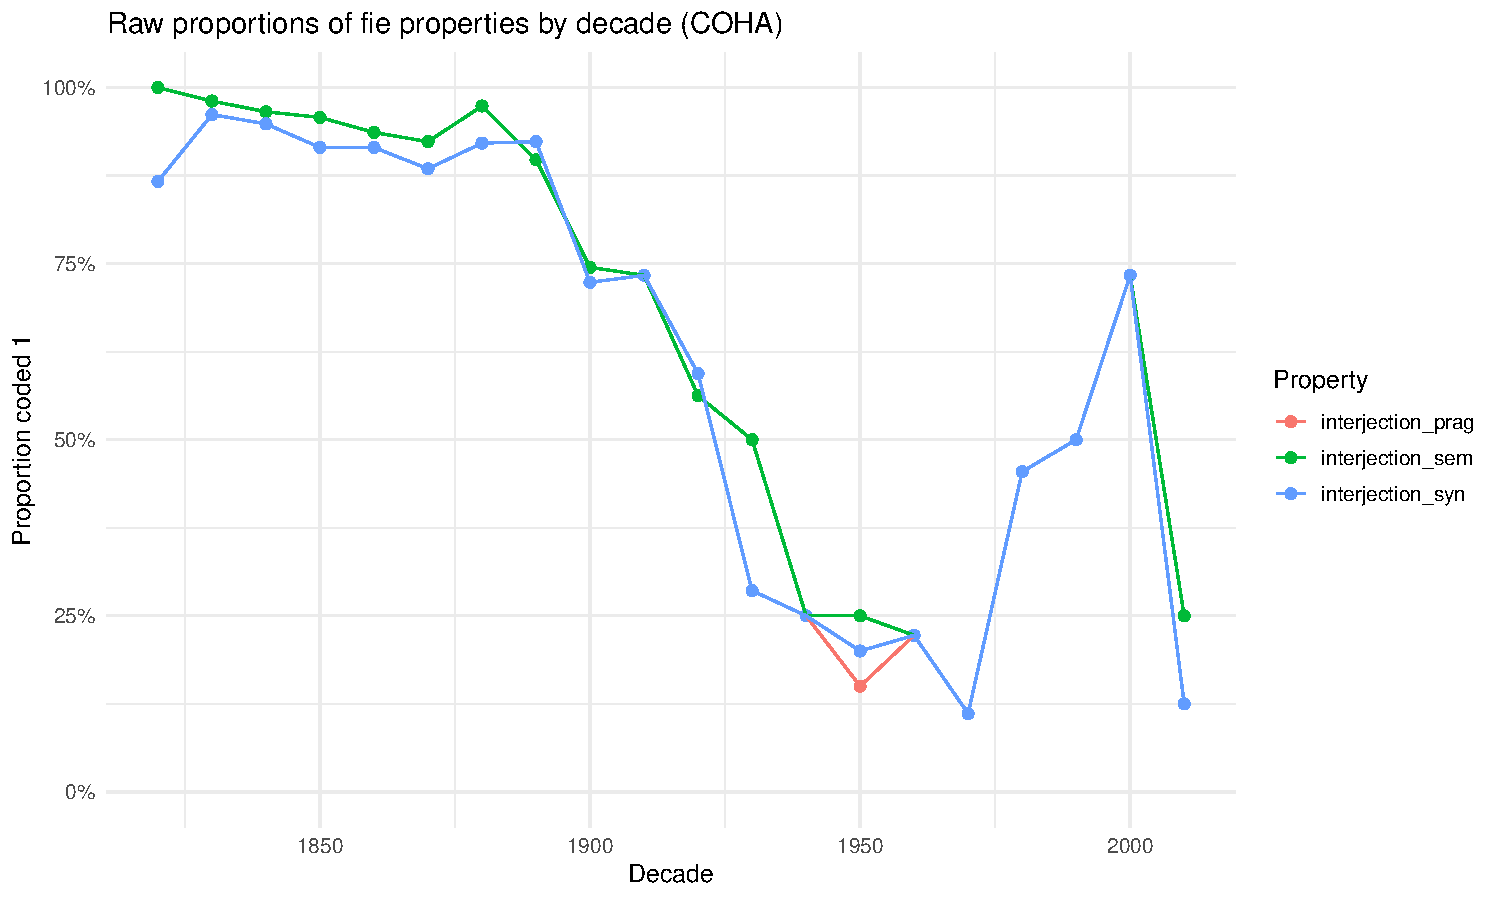
\includegraphics[width=.82\textwidth]{fie-raw-proportions.pdf}
  \caption{Archived proportions coded~1 by decade in the 616-row \mention{fie} input (COHA, 1820--2019). These are the original diagnostic trajectories, retained to document the attempted analysis. Because OCR substitutions remain in their denominator as zero-valued observations, the curves aren't interpreted as estimates of linguistic property loss.}
  \label{fig:fie-raw}
\end{figure}

\subsection{Archived models and interpretation}

The script fits three separate decade-level binomial logistic regressions, with time centred and scaled in ten-year units. Its normal priors have mean zero and standard deviations 1.5 for the intercept and 0.5 for the slope, with the latter restricted to negative values. Each fit uses four chains, 2,000 warmup and 2,000 subsequent iterations per chain, and seed 2026. The negative-slope restriction imposes monotonic decline and can't model revival. Separate likelihoods also leave the three outcomes' within-token dependence unmodelled.

The script centres decade labels rather than the midpoints specified in the preregistration. Because centring cancels a common offset, this discrepancy leaves the fitted predictor and the ordering probability unchanged. It shifts the conversion back to calendar dates by approximately five years. This bookkeeping issue is separate from the invalid denominator, which blocks the substantive interpretation.

\begin{samepage}
The reported ED50 dates ($\tau$, the 0.5 probability crossing) were:

\begin{center}
\begin{tabular}{lrr}
  \hline
  Diagnostic & $\tau$ (median) & 95\% CrI \\
  \hline
  \intj{syn} & 1947 & 1937--1958 \\
  \intj{prag} & 1948 & 1939--1959 \\
  \intj{sem} & 1949 & 1941--1960 \\
  \hline
\end{tabular}
\end{center}
\end{samepage}

The archived probability of $\tau_{\text{int}} < \tau_{\text{sem}} < \tau_{\text{syn}}$ is 0.13, below the preregistration's informal 0.25 threshold for \enquote{inconsistent}. Identical independent priors assign each strict ordering probability $1/6$, so 0.13 wouldn't itself be strong evidence against this order even with a valid denominator. Marginal interval overlap wouldn't establish equality or simultaneity either. More fundamentally, the measurement audit supersedes the substantive interpretation of all these outputs: they supply no present test for or against ordered erosion.

\begin{figure}[ht]
  \centering
  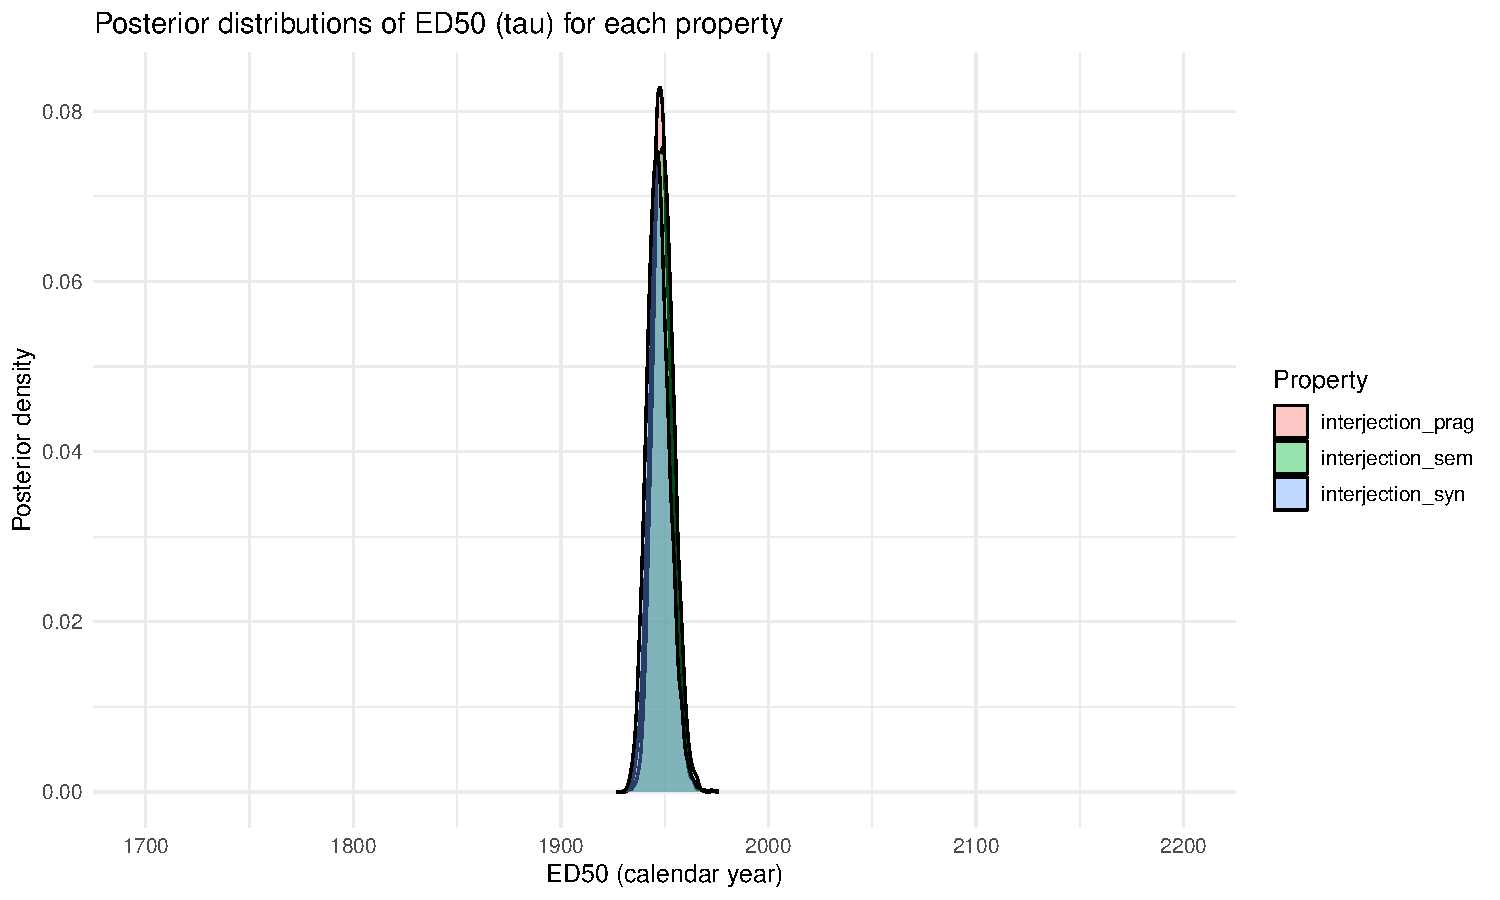
\includegraphics[width=.86\textwidth]{fie-tau-posteriors.pdf}
  \caption{Archived ED50 distributions from an analysis whose input failed the preregistered exclusion rule. The numerical outputs are retained for the audit record; their overlap isn't evidence for simultaneous loss, and the distributions aren't interpreted as valid estimates of linguistic erosion.}
  \label{fig:fie-tau}
\end{figure}

The audit is tied to repository revision \texttt{074dfb44cef5b18d292ac176ba5acbfedc76e3b1}, especially \path{fie-coha-preregistration.md}, \path{analysis/fie-confirmatory-model.R}, \path{analysis/fie-coding-sheet-annotated.csv}, and \path{analysis/fie-excluded.csv}. A valid comparison would first distinguish eligible occurrences from noise, then separate changing mixtures of sign-types from diagnostic change conditional on a bearer. No recoding or replacement model is reported here.


\clearpage
\section{Turnover in the tagged COHA inventory}
\label{app:turnover}

The Corpus of Historical American English (COHA) inventory supplies a descriptive result
\citep{davies2010}. In the 1820s, the six most frequent interjection-tagged
lemmas are \mention{no}, \mention{oh}, \mention{yes}, \mention{nay},
\mention{o}, and \mention{ah}. In the 2010s, \mention{yeah}, \mention{hey},
and \mention{uh} occupy three of those places. The change concerns
frequency ranks: displaced forms needn't disappear, and the tagging
policy doesn't independently identify the inquiry-relative categories.

The retained \mention{no}, \mention{oh}, and \mention{yes} share their
high ranks across the two periods, but inventory turnover alone
doesn't show persistence of a grammatical, semantic, or interactional
profile. That would require comparable diagnostics of the relevant
uses over time. Figure~\ref{fig:turnover} preserves the descriptive
result, whose evidential contribution is the changing recorded inventory.

\begin{figure}[htbp]
  \centering
  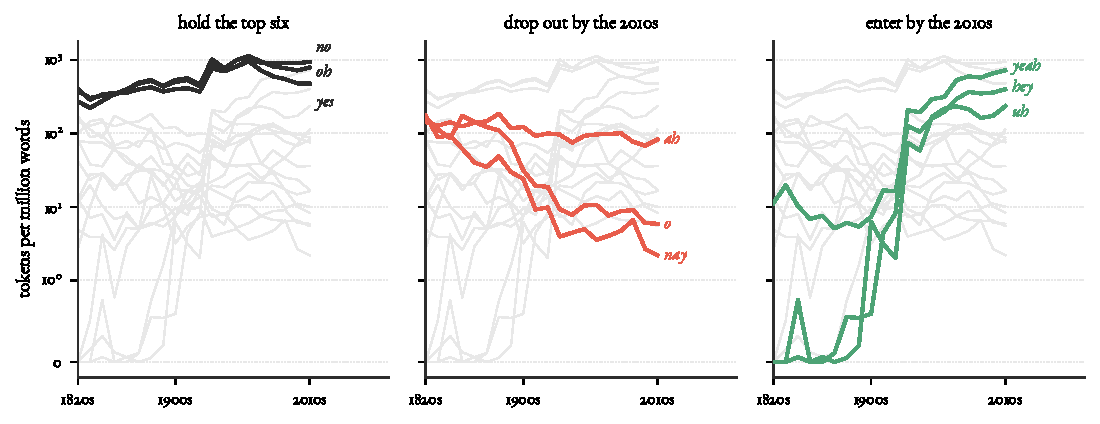
\includegraphics[width=\textwidth]{interjection-turnover.pdf}
  \caption{Turnover in the COHA interjection-tagged inventory. Each panel
  shows the twenty most frequent tagged lemmas across the corpus in grey,
  with one group highlighted. Three of the 1820s top six are displaced
  in that ranking by the 2010s. Frequencies per million words use a
  symmetric log scale retaining zeros. These rankings don't measure
  stability of a grammatical, semantic, or interactional profile.}
  \label{fig:turnover}
\end{figure}

The frequencies were extracted on 27 July 2026 and archived under
\path{analysis/hand-extracted/}. The 1820s ranking uses the complete
111-form tagged list for that decade, rather than restricting the
comparison to the all-period top twenty. This preserves a valid
comparison of ranks while leaving the separate question of what
the tag includes open to measurement audit.


\clearpage
\printbibliography
\end{document}
